\newpage
\section{Design and Implementation}
\label{sec:designandimplementation}

\begin{enumerate}[label=\Alph*.]
    \item System Block Diagram
    \label{subsec:systemblockdiagram}

    \hspace*{1em} The designed system has several main components: the sensor part, the control part, the mechanical system part, and the motion data part.

    \begin{figure} [h] \centering
        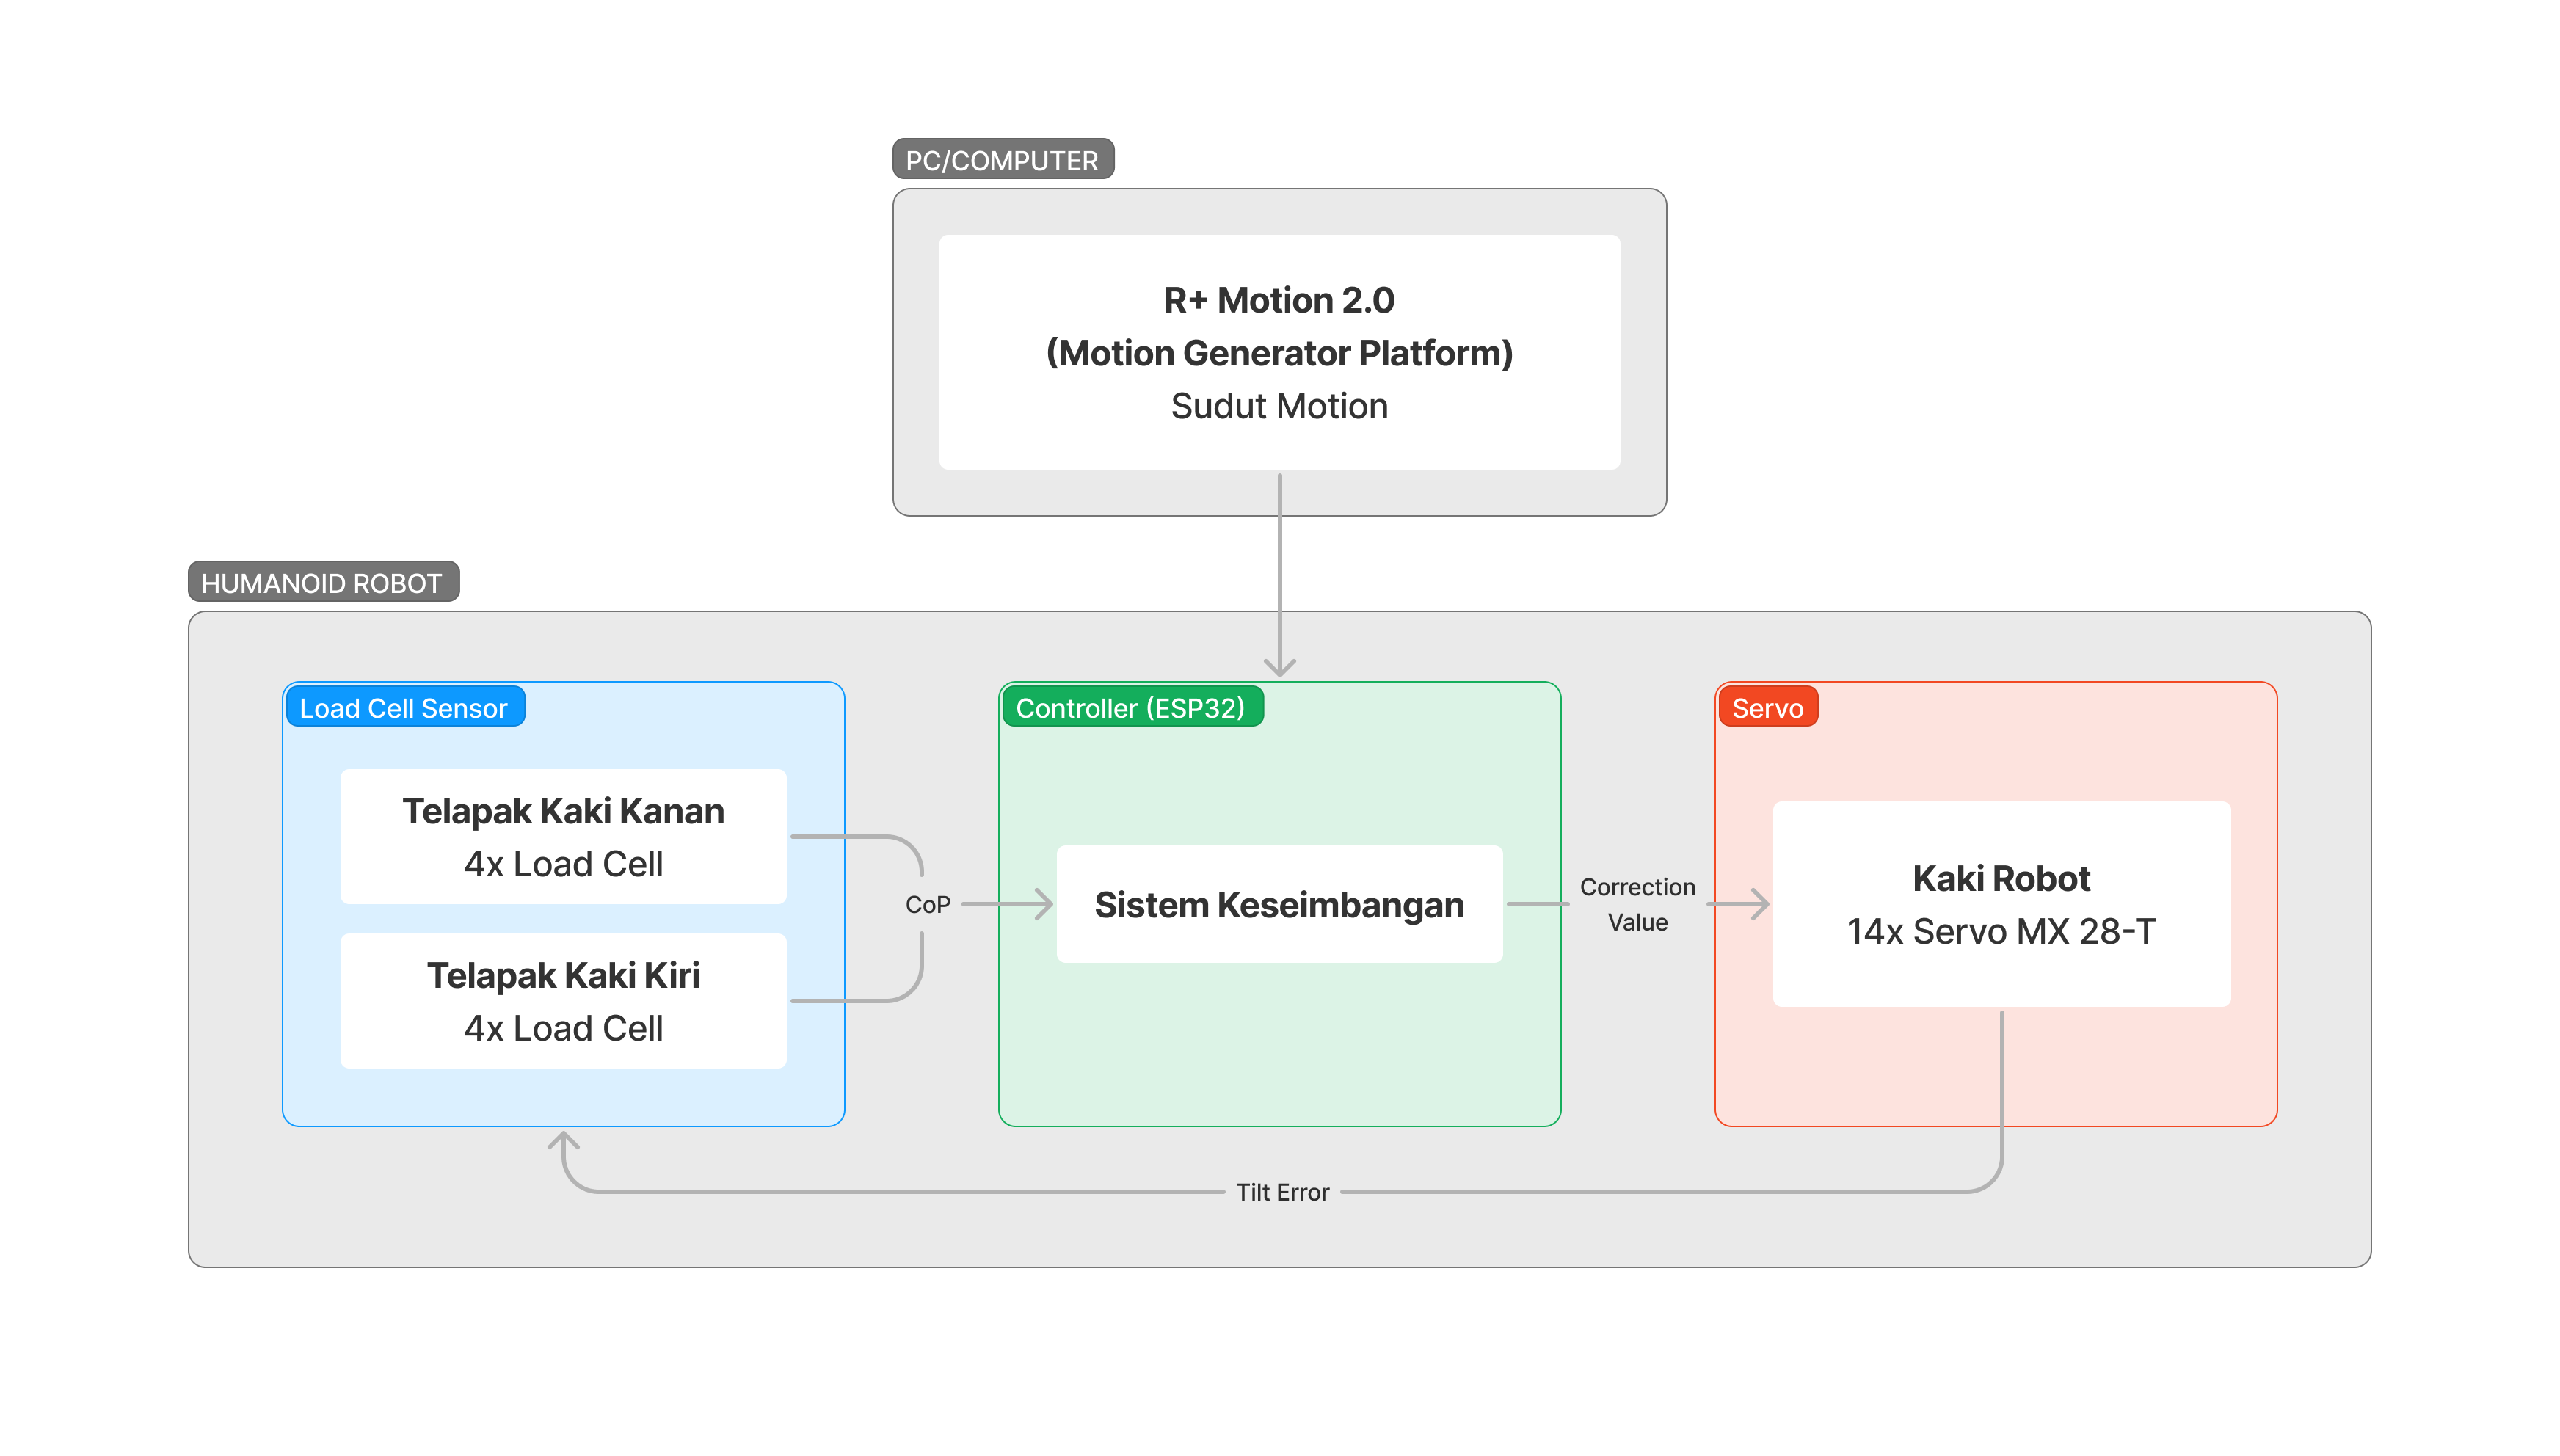
\includegraphics[width=0.45\textwidth]{gambar/Diagram_Sistem.png}
        \caption{Overall System Diagram}
        \label{fig:Diagram_Sistem}
    \end{figure}
    
    \hspace*{1em} The sensor part includes load cells mounted on each foot of the robot. These load cells detect the load or pressure on the robot's feet. The control part involves a microcontroller responsible for processing data from the sensors and controlling the robot's movements. The mechanical system part includes the robot's frame consisting of various servos used to move the robot. The motion data part stores pre-designed movements in the microcontroller's file system. This data consists of several frames containing an array of target positions for each servo along with the time required to reach those positions. The system diagram can be seen in Figure \ref{fig:Diagram_Sistem}.

    \item Mechanical System
    \label{subsec:mechanicalsystem}

    \hspace*{1em} The design of the humanoid robot body includes 29 degrees of freedom. The upper body uses 15 XL-320 type servos, while the lower body uses 14 MX-28 type servos. The detailed design, dimensions, and servo ID naming on the robot can be seen in Figure \ref{fig:Desain_Mekanik}. 

    \begin{figure} [h] \centering
      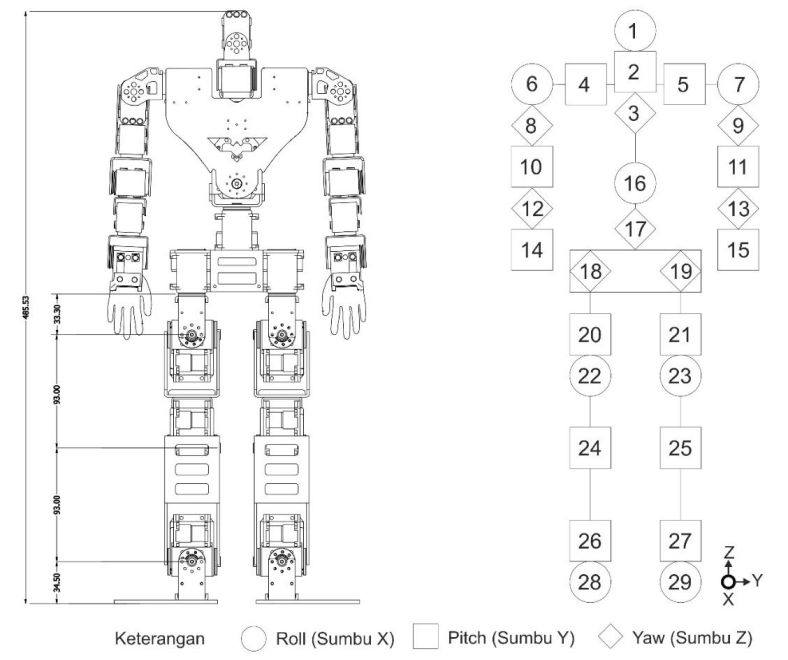
\includegraphics[width=0.35\textwidth]{gambar/Desain_Mekanik.png}
      \caption{Mechanical Design of the Robot and Servo ID Naming}
      \label{fig:Desain_Mekanik}
    \end{figure}

    \item Electronic System
    \label{subsec:electronicsystem}

    \hspace*{1em} The hardware system in this research is explained through the block diagram shown in Figure \ref{fig:Diagram_Elektronik}. This system uses an embedded system consisting of ESP32 and ESP32-C3 microcontrollers. The embedded system was chosen because the robot developed in this research is an improvement from previous research conducted by Fahd (2018)\cite{fahd}.

    \begin{figure} [h] \centering
      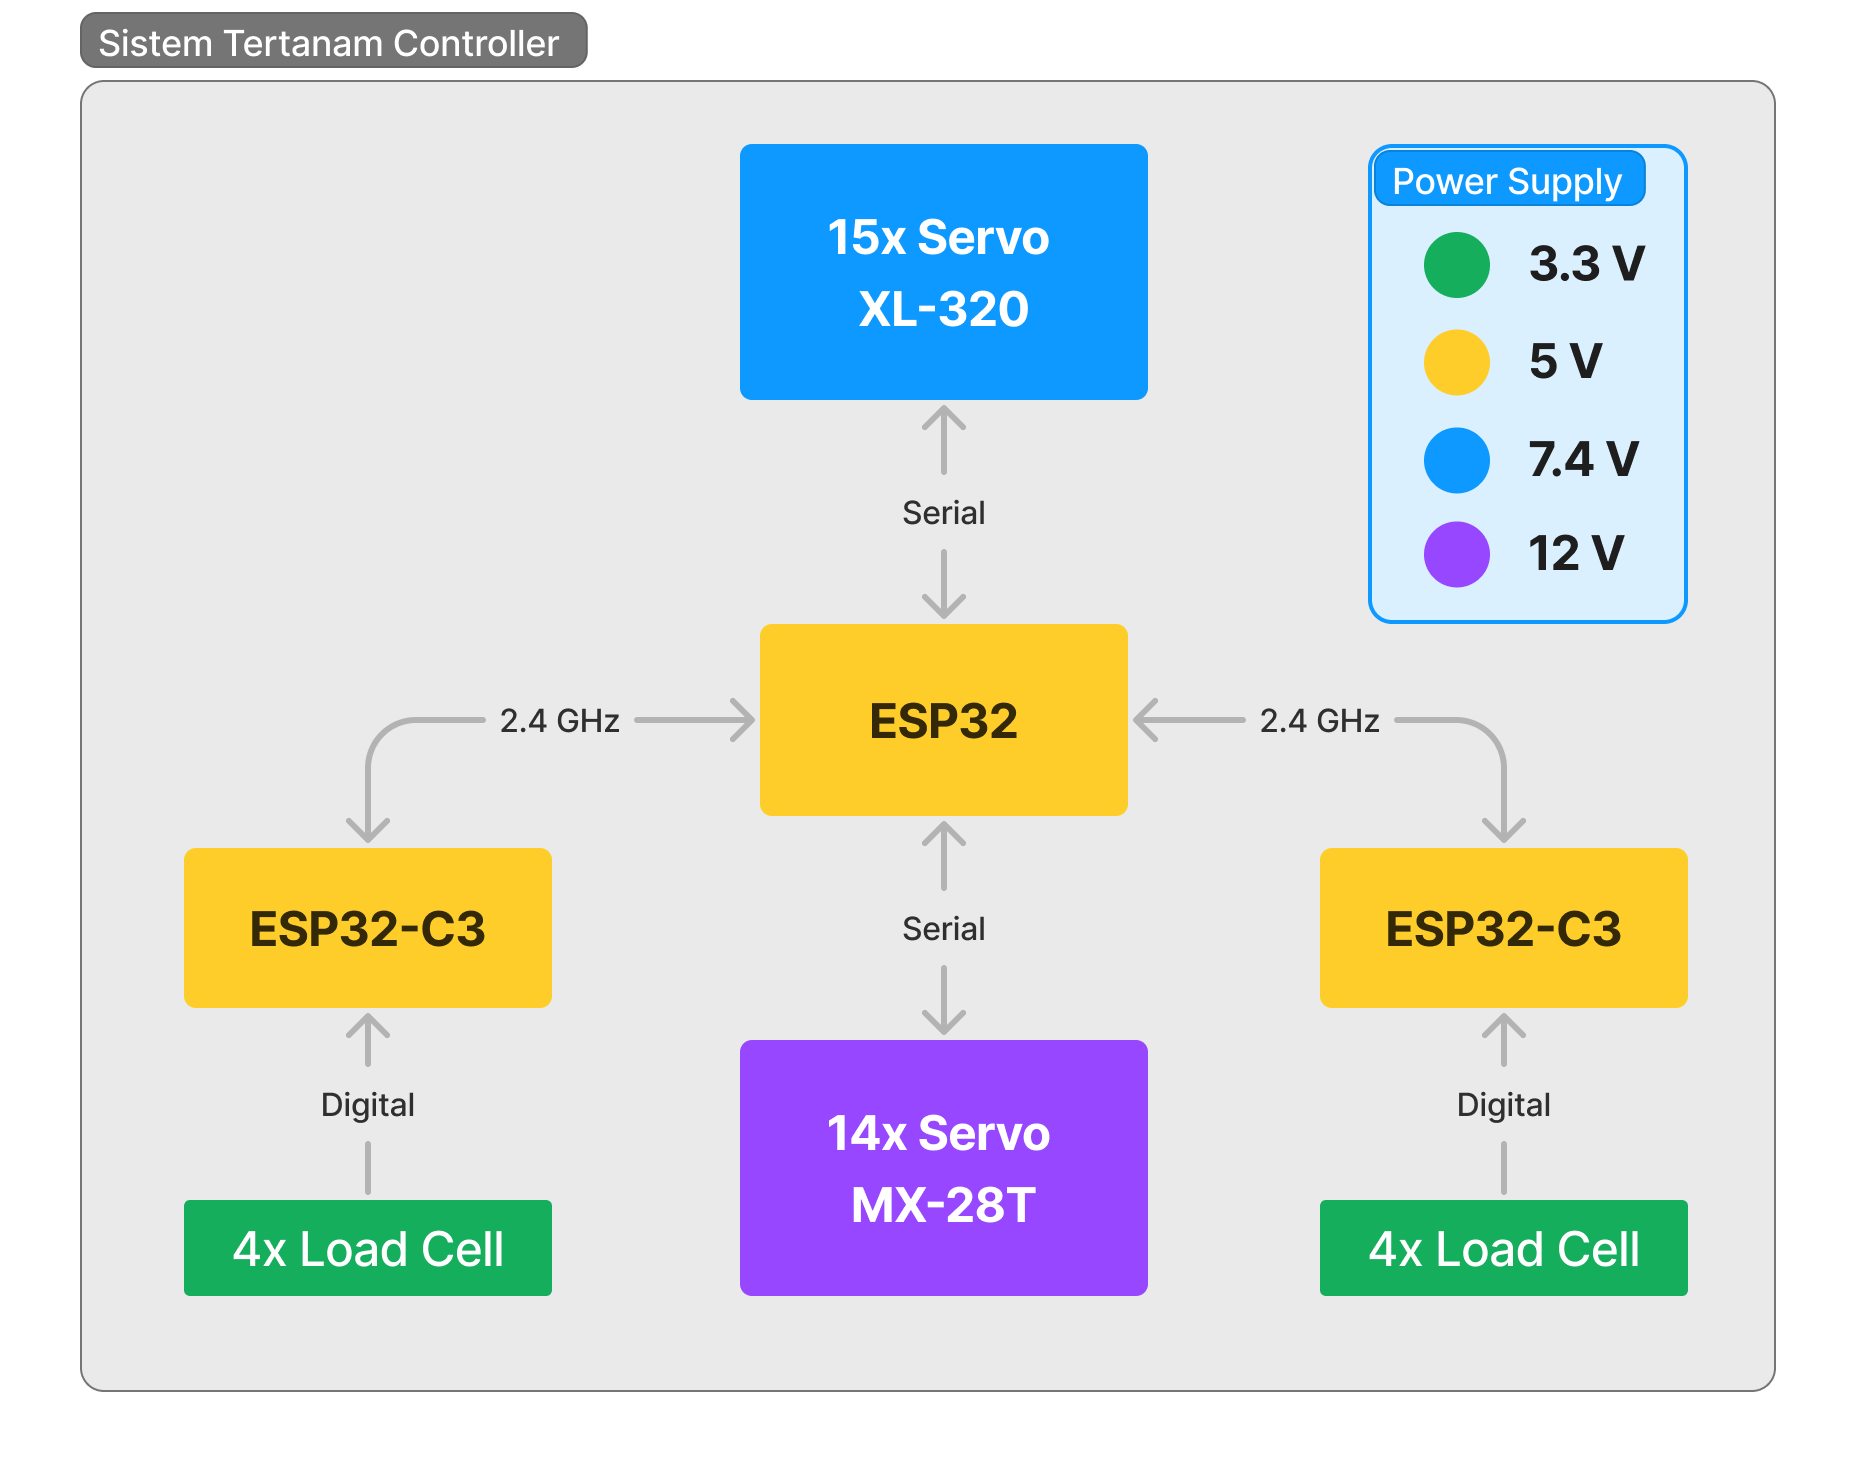
\includegraphics[width=0.4\textwidth]{gambar/Diagram_Elektronik.png}
      \caption{Electronic and Communication Diagram Between Components}
      \label{fig:Diagram_Elektronik}
    \end{figure}

    \hspace*{1em} ESP32-C3 is used for data acquisition from the load cell and sends it to the ESP32. ESP32-C3 has the same Wi-Fi capability as ESP32, allowing wireless communication between the two microcontrollers. ESP32-C3 also has a smaller dimension, making it easier to be placed on the robot's foot.

    \item Foot Design of the Robot
    \label{subsec:desaignsystemloadcell}

    \hspace*{1em} Each robot foot is equipped with 4 load cells mounted at the ends of the foot. Each load cell detects pressure, allowing the system to determine the center of pressure on the robot's foot. The design of the robot foot can be seen in Figure \ref{fig:Desain_Kaki}.
    
    \begin{figure} [h] \centering
      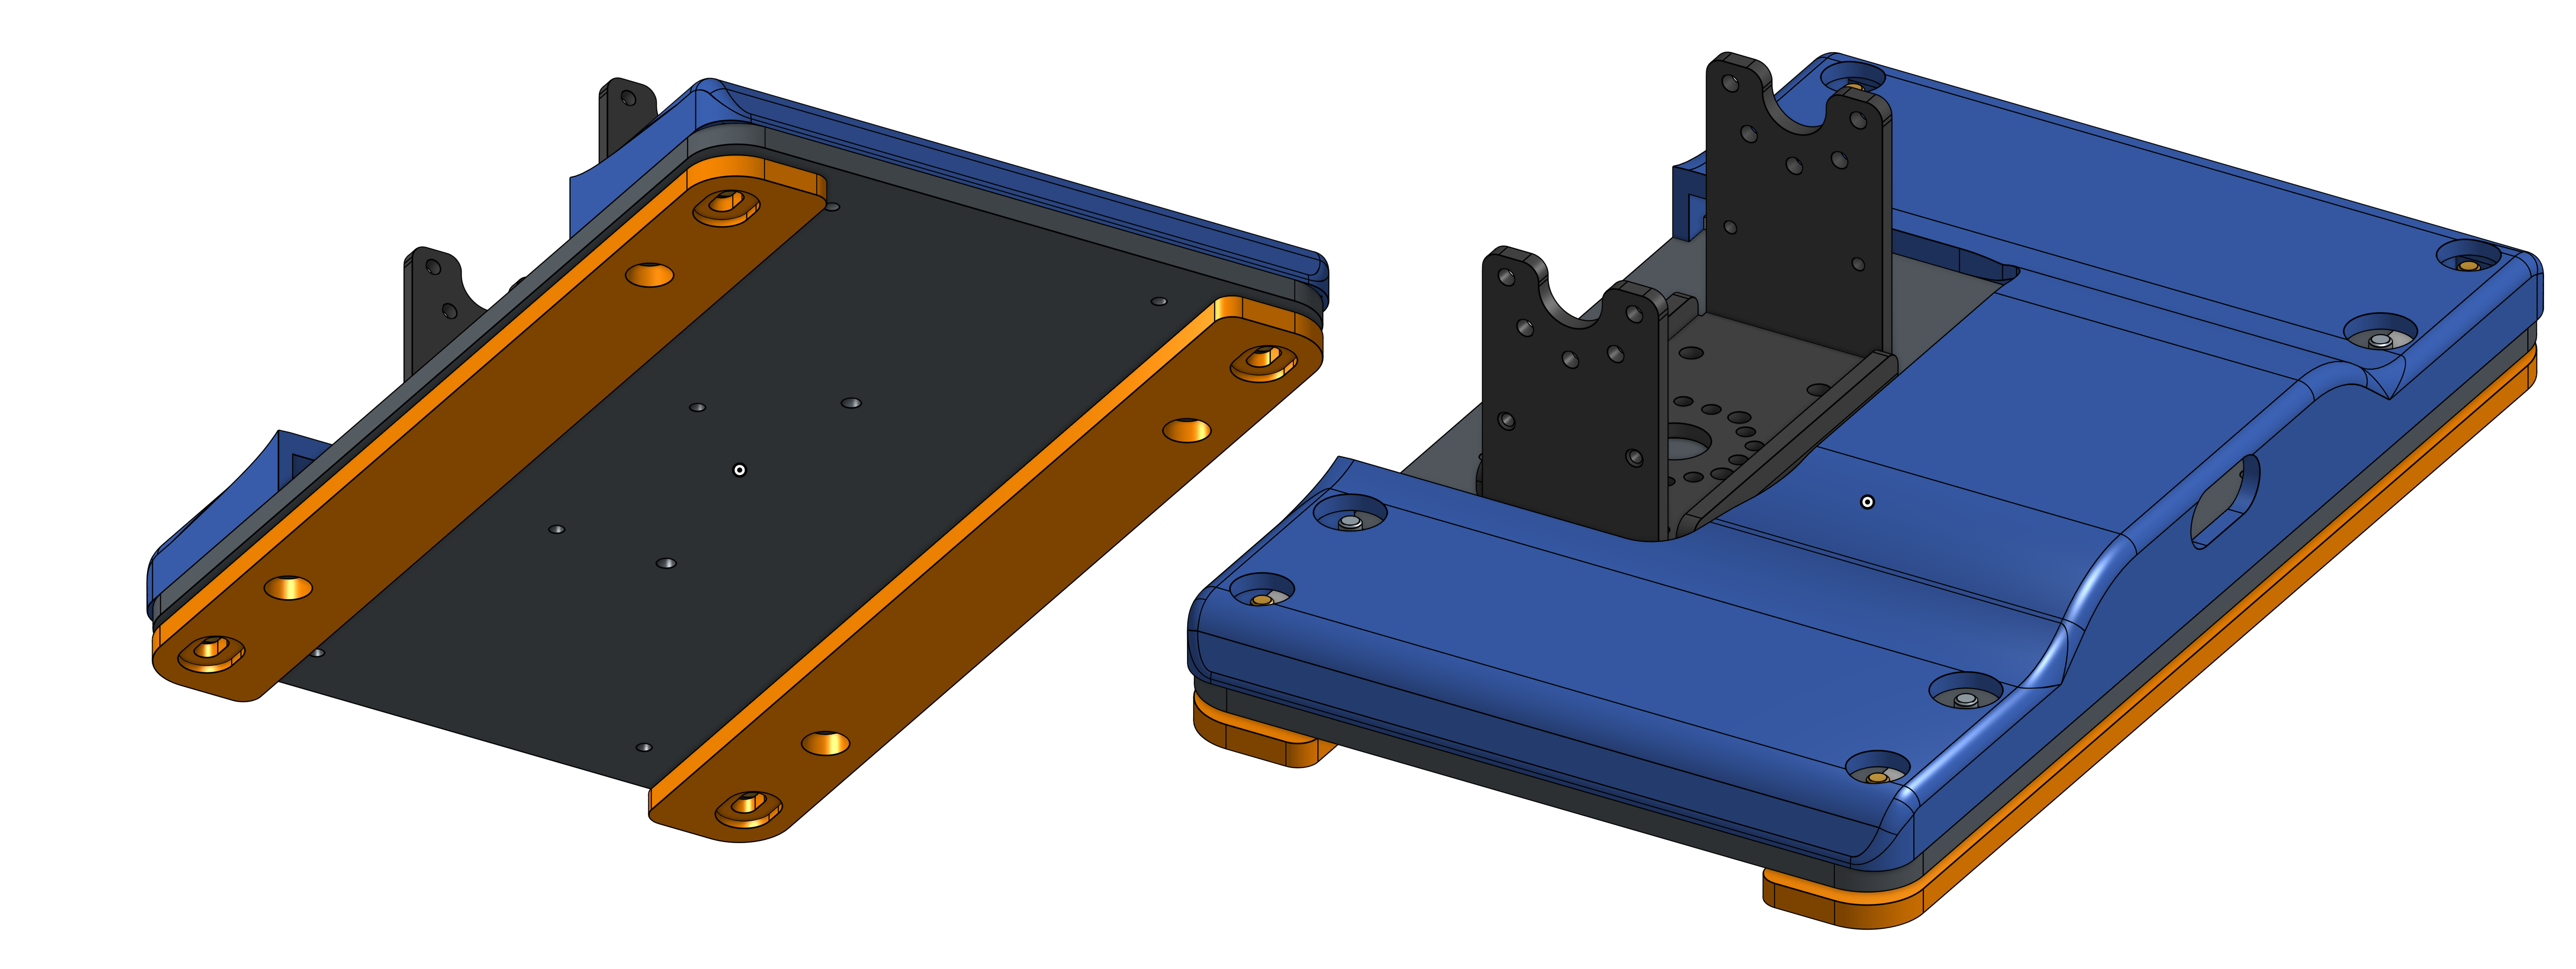
\includegraphics[width=0.4\textwidth]{gambar/Desain_Kaki.png}
      \caption{Overall Design of the Robot Foot}
      \label{fig:Desain_Kaki}
    \end{figure}

    \hspace*{1em} In Figure \ref{fig:Desain_Kaki}, it is shown that each load cell is placed at the end of the robot's foot. The load cells are connected to a microcontroller located inside the robot's foot. For the electronics part, a closure made from 3D print is provided to protect the components from damage. For the mechanical part, the load cell sensors are equipped with pads that serve as pressure points for the load cells and also provide anti-slip to prevent slipping.

    \item Load Cell Coefficient Configuration
    \label{subsec:configurationcoefficient}

    \hspace*{1em} Before the load cells can be used, calibration is necessary to measure the load cell coefficients by adjusting parameters such as scaling and offset values. To facilitate configuration, a graphical user interface (GUI) application was created, which is user-friendly and can be accessed through a browser. This GUI has a control menu for accessing functions and settings, and displays the center of pressure to visualize the impact of parameter changes on the system. Figure \ref{fig:Preview_Aplikasi} shows the configuration application interface, including the control menu and center of pressure display. This application will save configuration data to the EEPROM memory of the microcontroller, so the data remains stored even when the microcontroller is turned off.

    \begin{figure} [h] \centering
      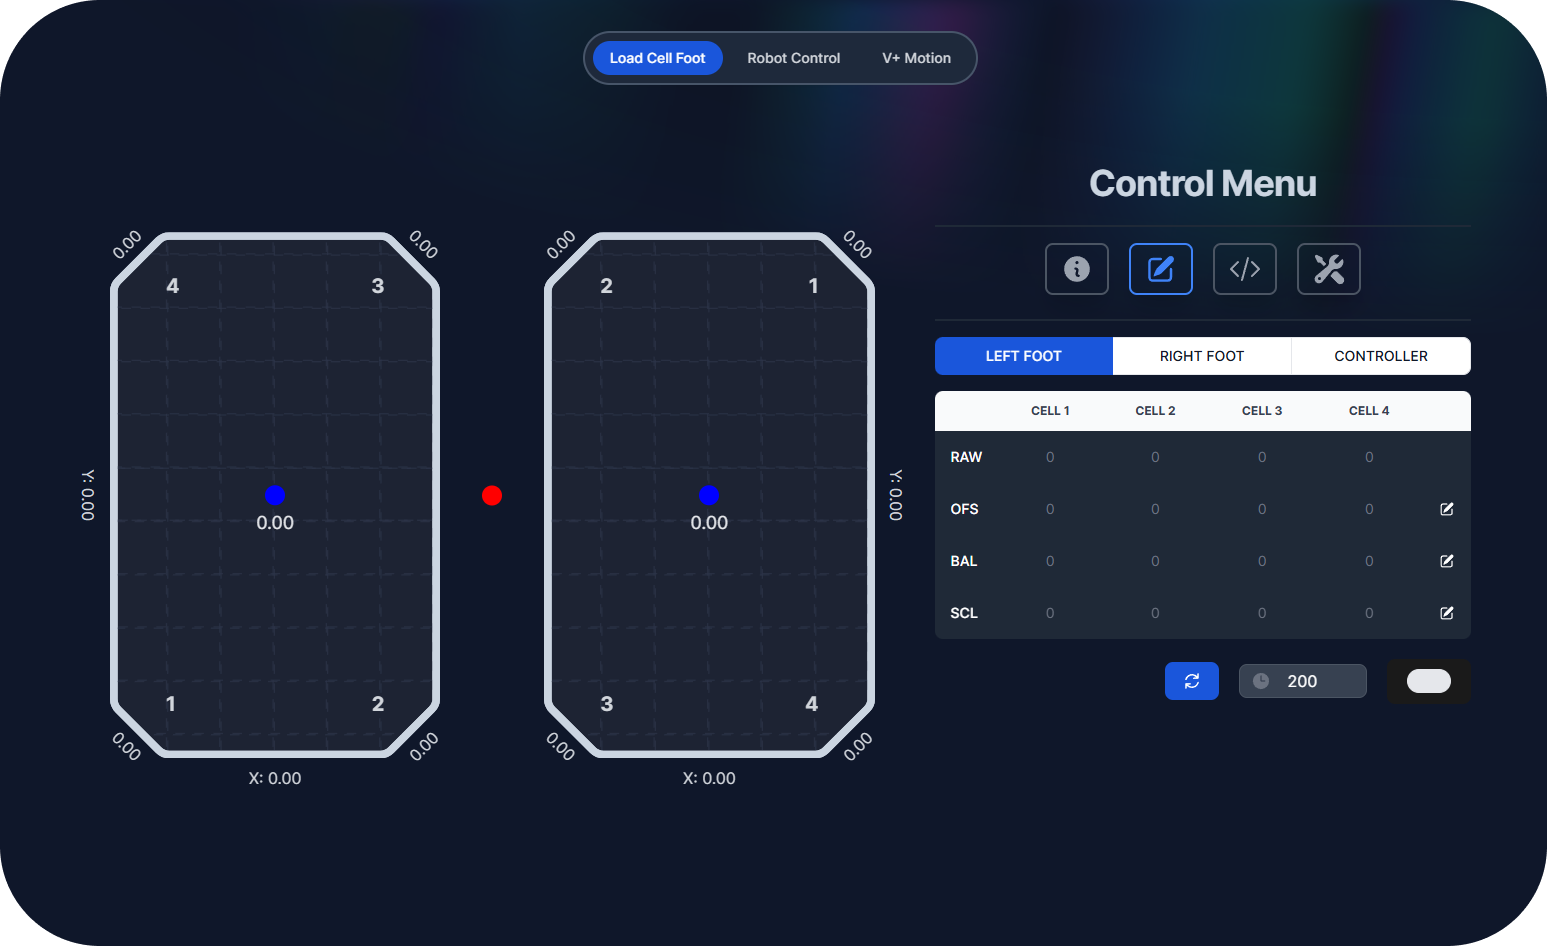
\includegraphics[width=0.4\textwidth]{gambar/preview_aplikasi.png}
      \caption{Application Used for Load Cell Configuration}
      \label{fig:Preview_Aplikasi}
    \end{figure}

    \item Center of Pressure Calculation for the Robot
    \label{subsec:pressurecentercalculation}

    \hspace*{1em} The center of pressure on the robot is calculated by combining data from both robot feet. The main microcontroller will communicate with the microcontrollers on the left and right feet to obtain the center of pressure and total pressure data. This data is then used to determine the position of the center of pressure relative to the robot. The calculation of the center of pressure position on the robot is done as shown in equations \ref{eq:Total_Force_Robot}, \ref{eq:COP_X_Robot}, and \ref{eq:COP_Y_Robot}.
    
    \begin{figure} [h] \centering
      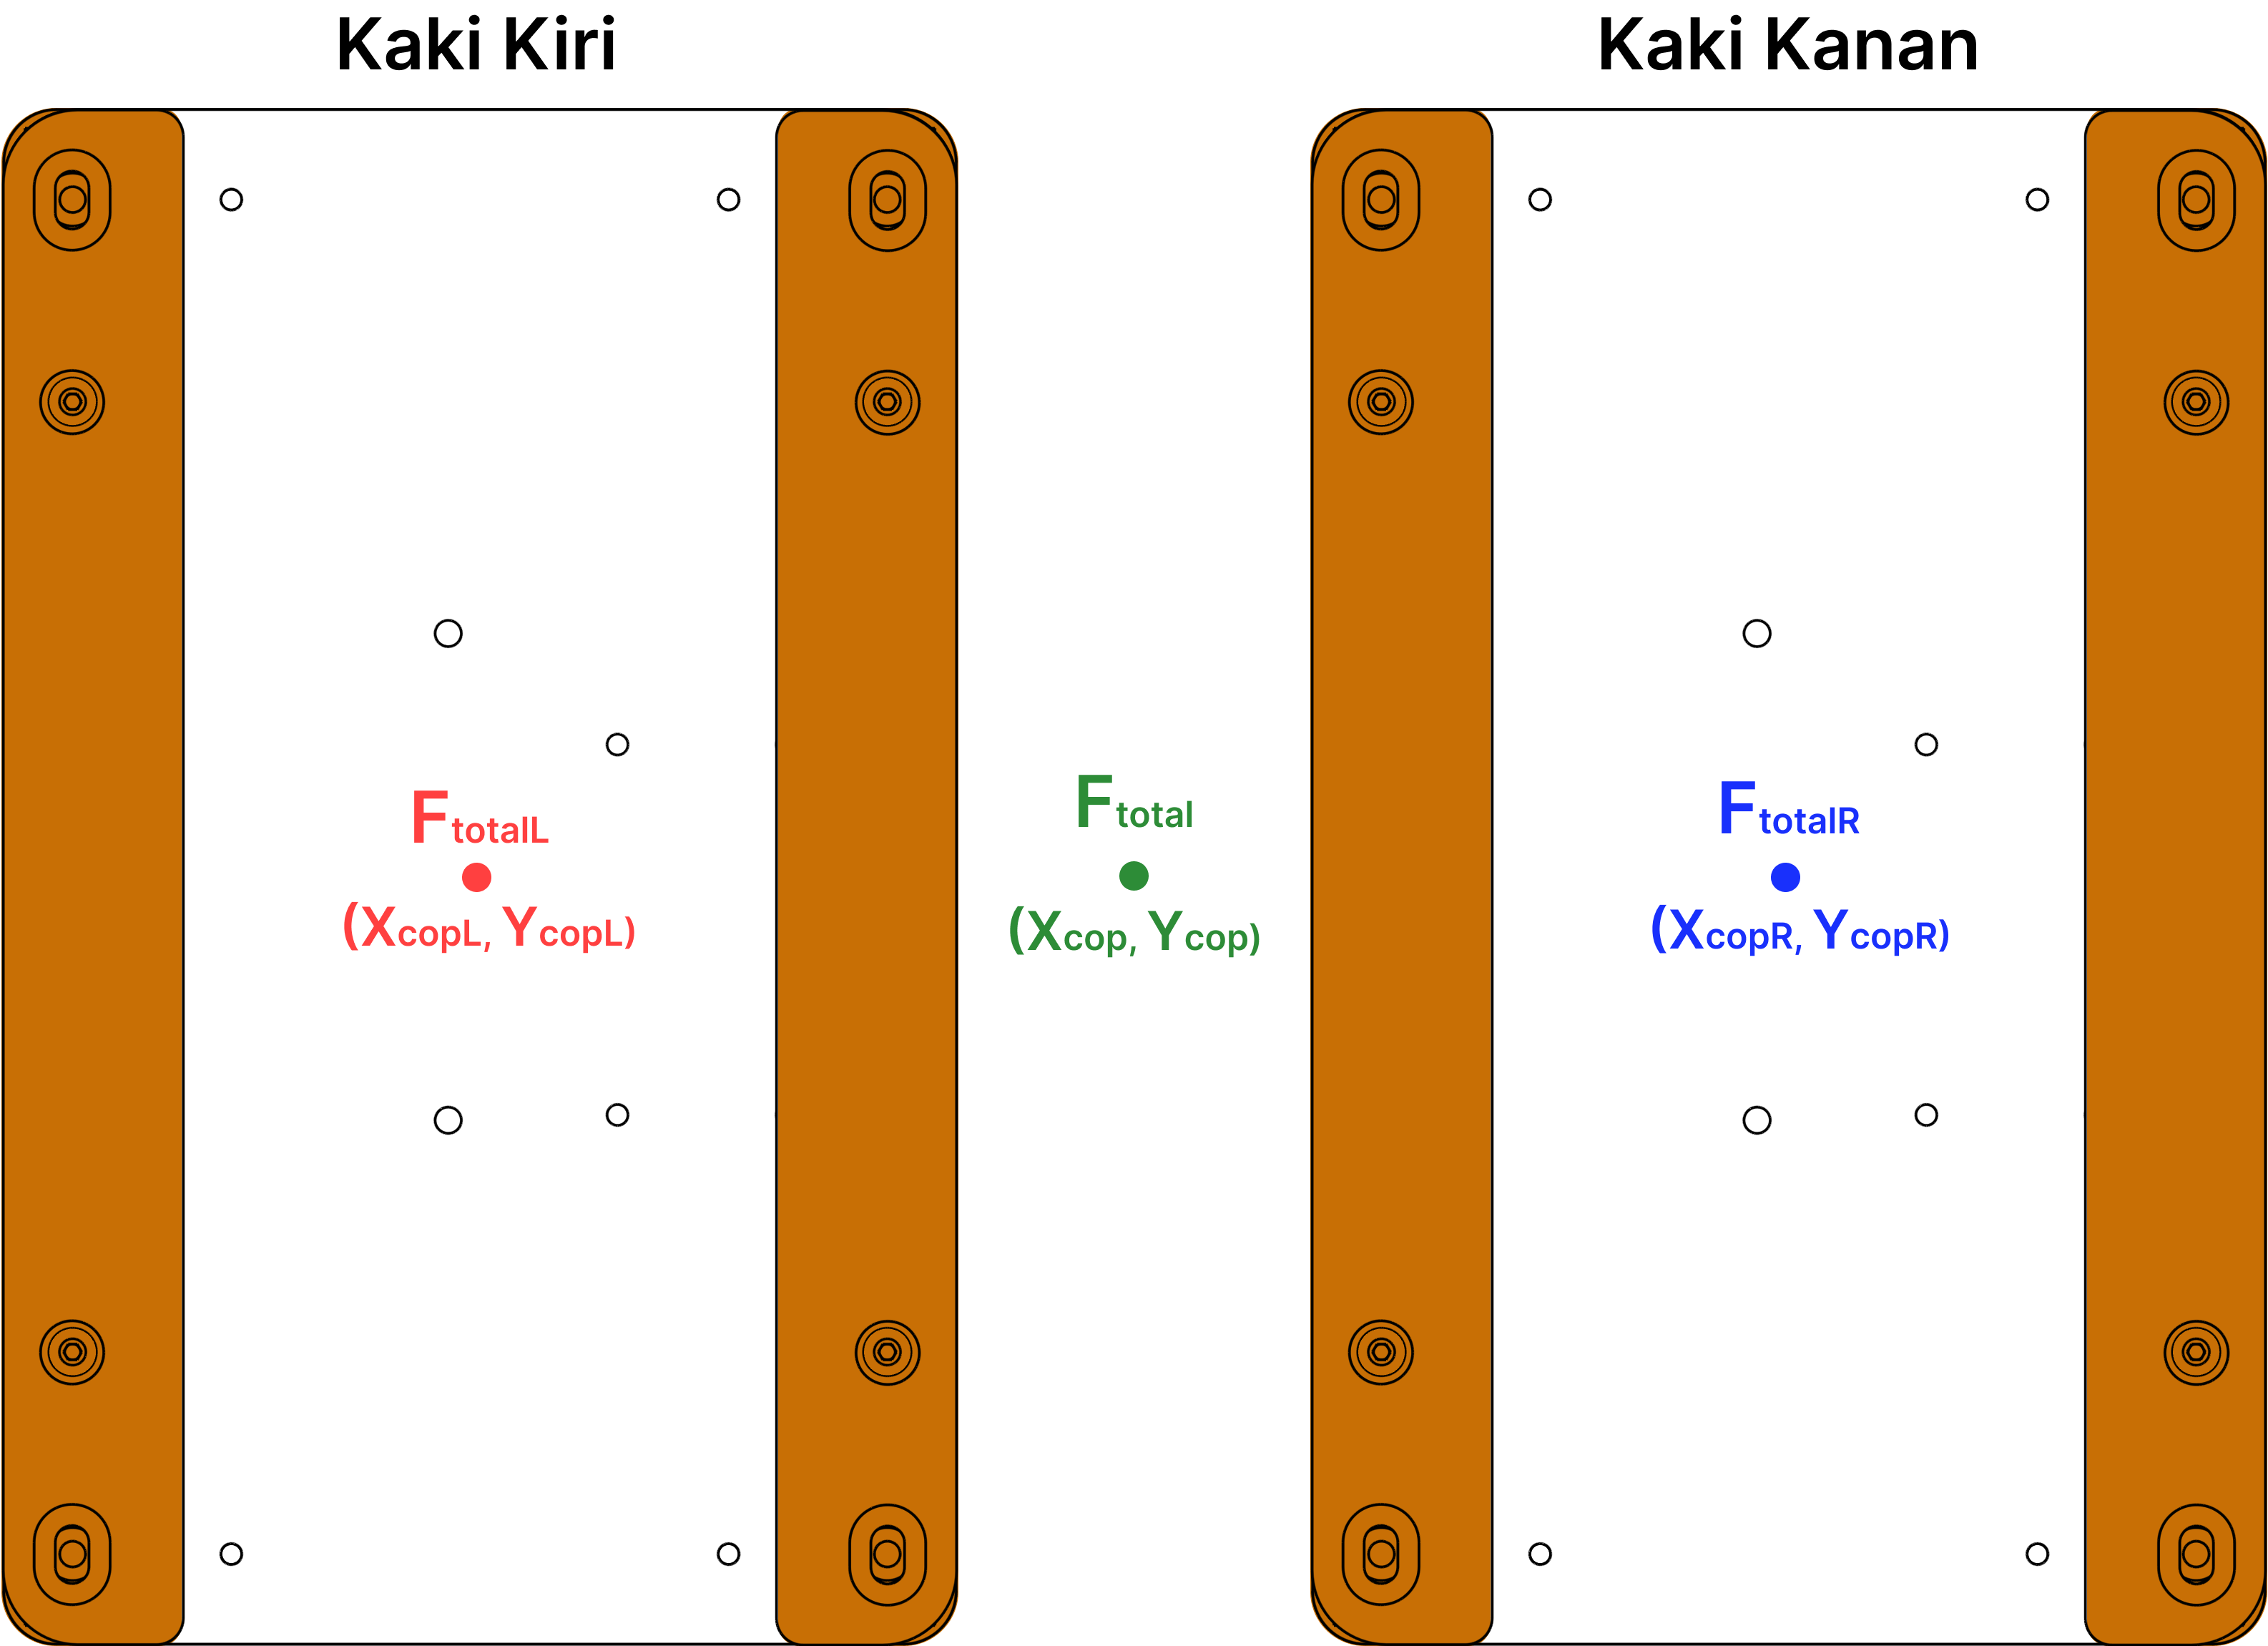
\includegraphics[width=0.4\textwidth]{gambar/COP_Robot.png}
      \caption{Center of Pressure on the Robot (Green), Center of Pressure on the Left Foot (Red), and Center of Pressure on the Right Foot (Blue)}
      \label{fig:COP_Robot}
    \end{figure}

    \begin{equation}
      F_{\mathrm{total}} = F_{\mathrm{totalL}} + F_{\mathrm{totalR}}
      \label{eq:Total_Force_Robot}
    \end{equation}

    \begin{equation}
      X_{\mathrm{cop}} = \frac{F_{\mathrm{totalL}} \cdot X_{\mathrm{copL}} + F_{\mathrm{totalR}} \cdot X_{\mathrm{copR}}}{F_{\mathrm{total}}}
      \label{eq:COP_X_Robot}
    \end{equation}

    \begin{equation}
      Y_{\mathrm{cop}} = \frac{F_{\mathrm{totalL}} \cdot Y_{\mathrm{copL}} + F_{\mathrm{totalR}} \cdot Y_{\mathrm{copR}}}{F_{\mathrm{total}}}
      \label{eq:COP_Y_Robot}
    \end{equation}

    \hspace*{1em} The center of pressure data in this study will use a scale. As shown in Figure \ref{fig:COP_Robot}, the Y-axis has a scale from -1 to 1. The upper limit is represented by the value 1, while the lower limit is represented by the value -1. The X-axis has a scale from -2 to 2, with the right limit represented by the value 2 and the left limit represented by the value -2. For the X-axis, when the robot's weight is supported on one foot, the center of pressure value will be positive or negative depending on the position of the supporting foot. When the robot is lifted, the center of pressure value will be at (0,0), which is in the middle of the foot.

    \item PID Control System Algorithm
    \label{subsec:pidcontrolalgorithm}

    \hspace*{1em} In this study, there are two PID controllers: the Pitch PID control and the Roll PID control. For the Pitch PID control, the input is the center of pressure position on the Y-axis. For the Roll PID control, the input is the center of pressure position on the X-axis. The setpoint for both the Pitch and Roll PID controls is the value obtained from the previous center of pressure input data. The error value is obtained from the difference between the current center of pressure position and the setpoint, as shown in Equation \ref{eq:Error_PID}, and the PID correction is calculated using Equation \ref{eq:Koreksi_PID}.

    \begin{equation}
      \mathrm{e} = COP_{\mathrm{error}} = COP_{\mathrm{set}} - COP_{\mathrm{input}}
      \label{eq:Error_PID}
    \end{equation}

    \begin{equation}
      \mathrm{Correction} = \mathrm{Kp} \cdot \mathrm{e} + \mathrm{Ki} \cdot \int \mathrm{e} + \mathrm{Kd} \cdot \frac{\mathrm{de}}{\mathrm{dt}}
      \label{eq:Koreksi_PID}
    \end{equation}

    \begin{figure} [h] \centering
      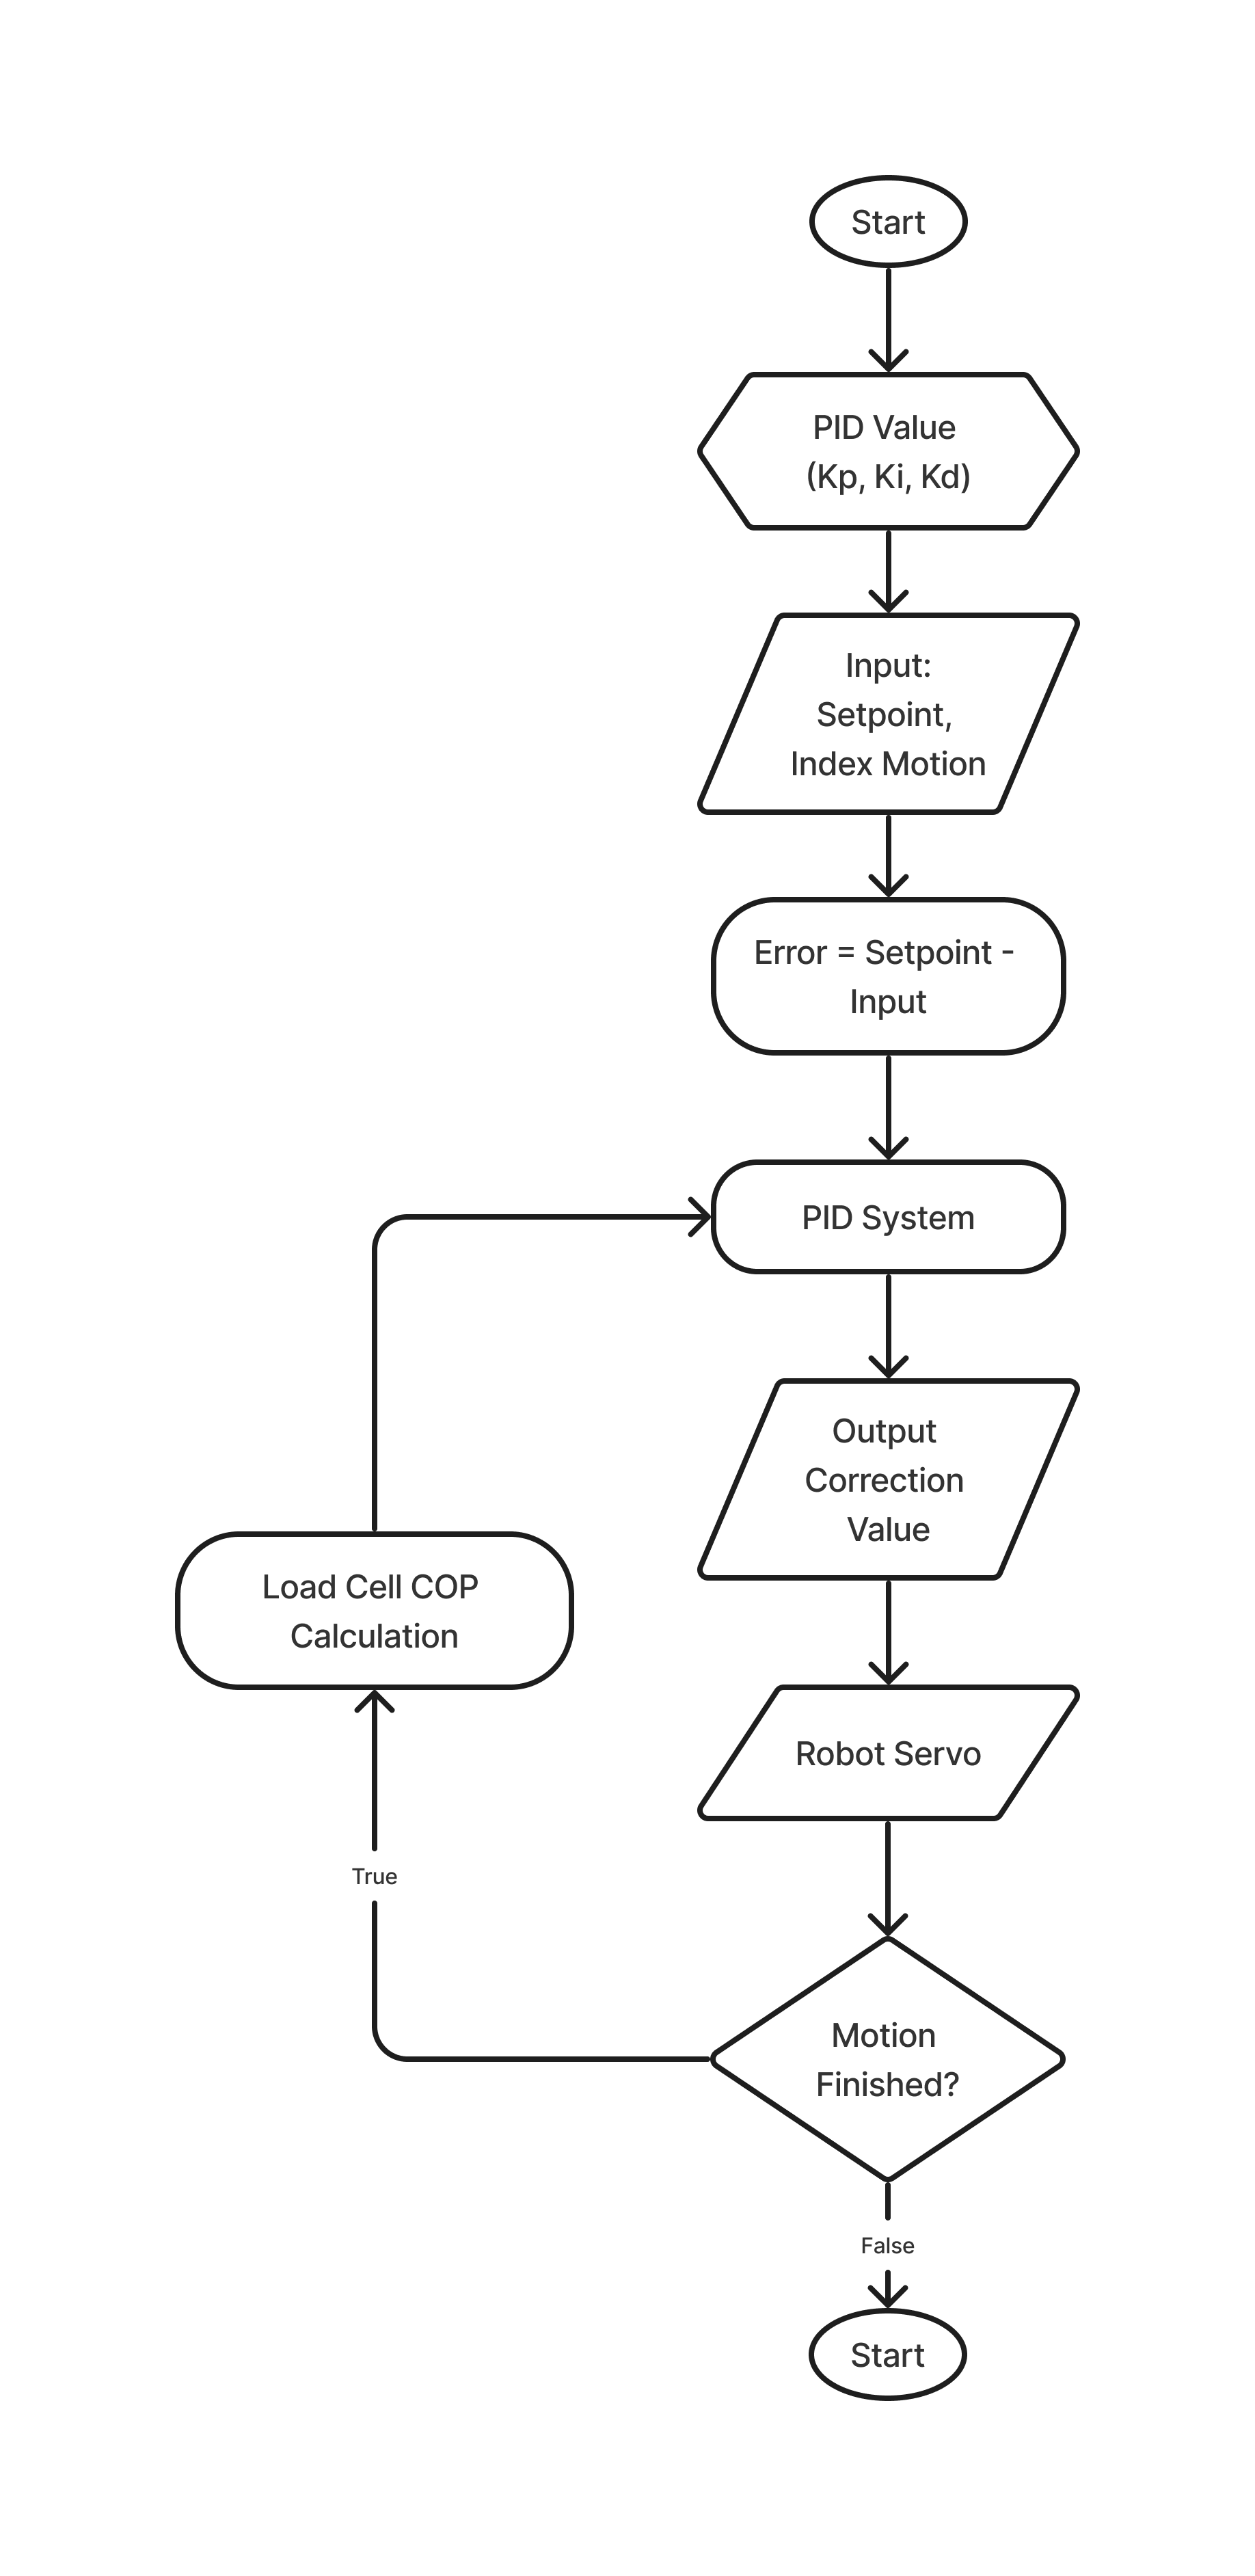
\includegraphics[width=0.38\textwidth]{gambar/Flow_Kontrol.png}
      \caption{PID Control System Flowchart When the Robot is in Motion}
      \label{fig:Flow_Kontrol}
    \end{figure}
    
    \hspace*{1em} The flowchart in Figure \ref{fig:Flow_Kontrol} shows the stages of the system's response to the error caused by the difference between the desired and actual center of pressure positions. First, the PID values are adjusted according to the system characteristics, then the setpoint is set to the desired center of pressure position. The error is calculated by subtracting the setpoint value from the input value using Equation \ref{eq:Error_PID}. This error value is used to compute the correction using Equation \ref{eq:Koreksi_PID}, which is then used to adjust the servo position as compensation. The robot will perform movements to maintain balance based on the correction produced by the PID control, which continues until the robot's motion is completed.

    \begin{figure} [h] \centering
      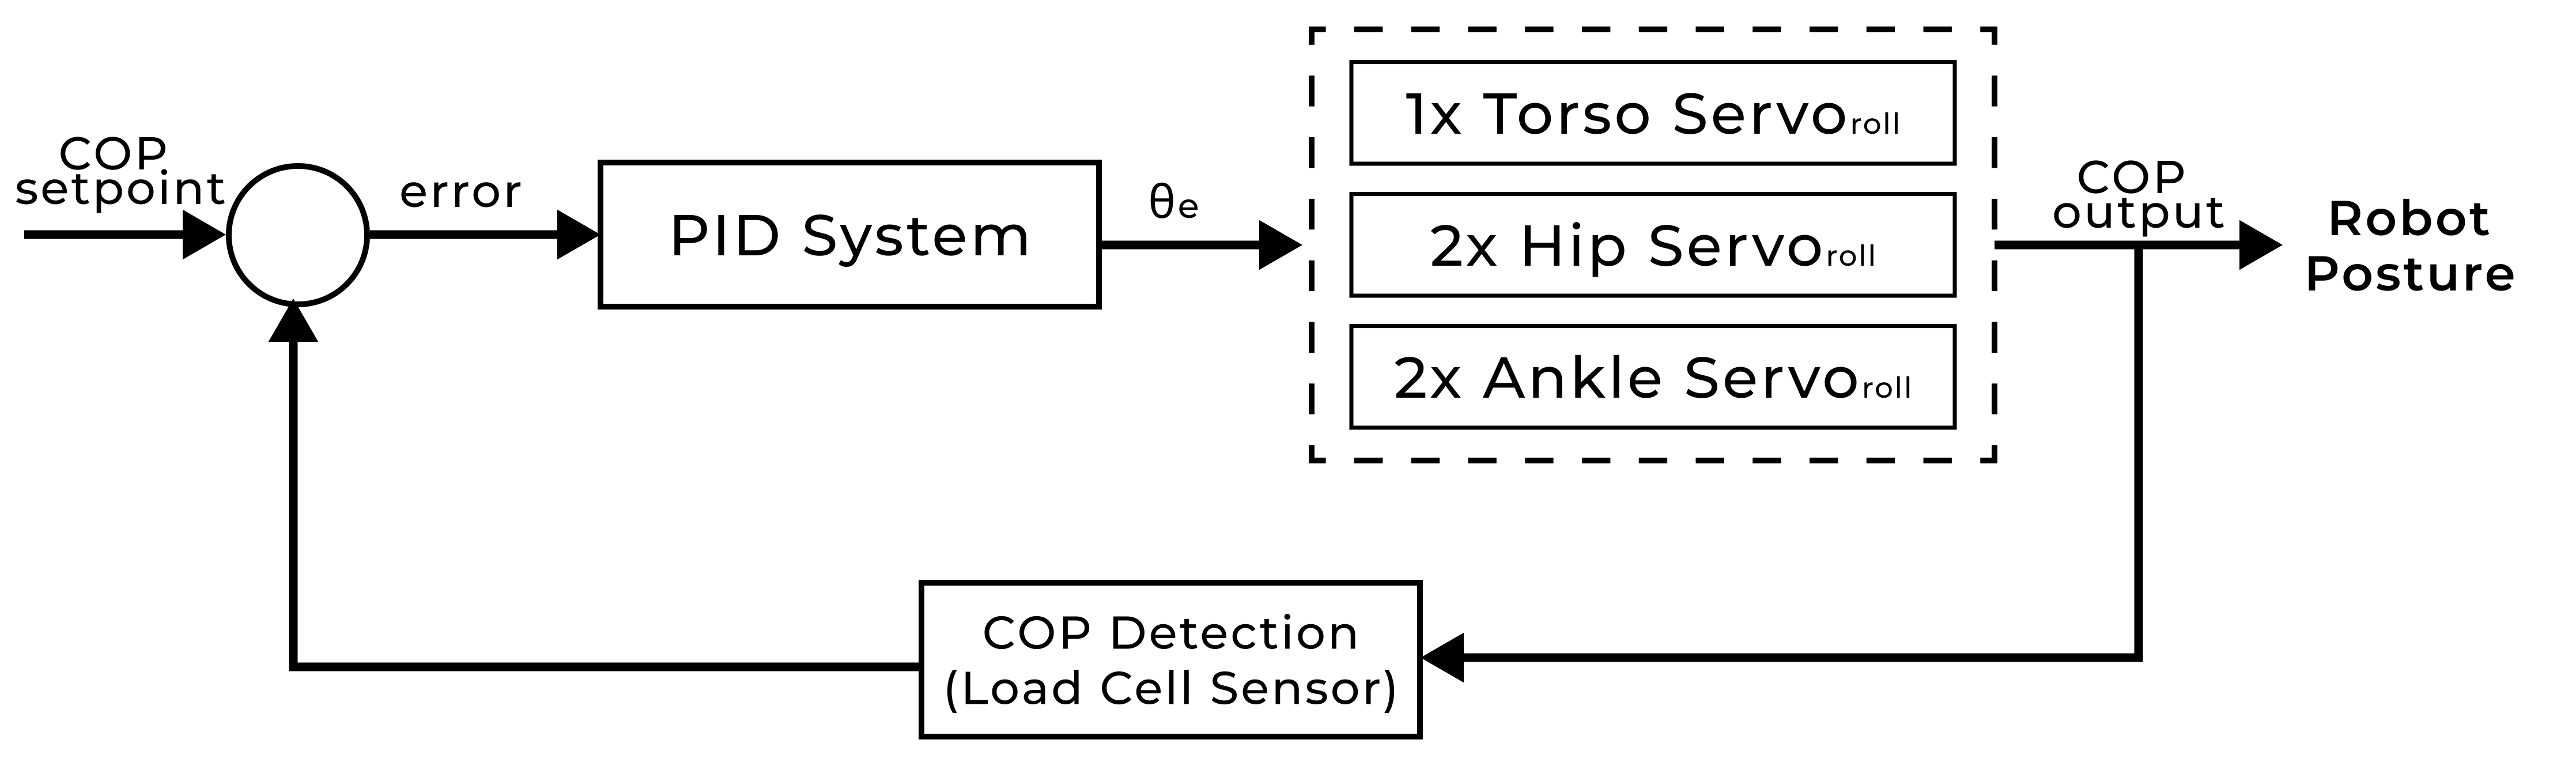
\includegraphics[width=0.4\textwidth]{gambar/pid_diagram.png}
      \caption{PID Control System Diagram}
      \label{fig:Control_System}
    \end{figure}

    \hspace*{1em} Figure \ref{fig:Control_System} shows the control system diagram consisting of three main blocks: the PID control block, the servo block as compensation, and the center of pressure block. The PID control block calculates the correction value based on the error between the desired and actual center of pressure positions. This correction value is used to adjust the servo position in the servo block as compensation. The center of pressure block calculates the center of pressure position on the robot's foot and provides this data as input to the PID control.

    \item Servo Adjustment for Compensation
    \label{subsec:servosettings}

    \hspace*{1em} In this study, the servo used to maintain balance is the one that adjusts the robot's roll position. These servos are located at the torso, hip, and ankle. By adjusting several servo angles, the robot can make necessary adjustments to maintain balance while moving or standing on uneven surfaces. Five servos are used, consisting of one servo at the torso (ID 1), two servos at each hip (ID 4 and ID 5), and two servos at each ankle (ID 13 and ID 14). The servo adjustment for compensation is shown in Figure \ref{fig:Controlled_Servo}, highlighted in blue.

    \begin{figure} [h] \centering
      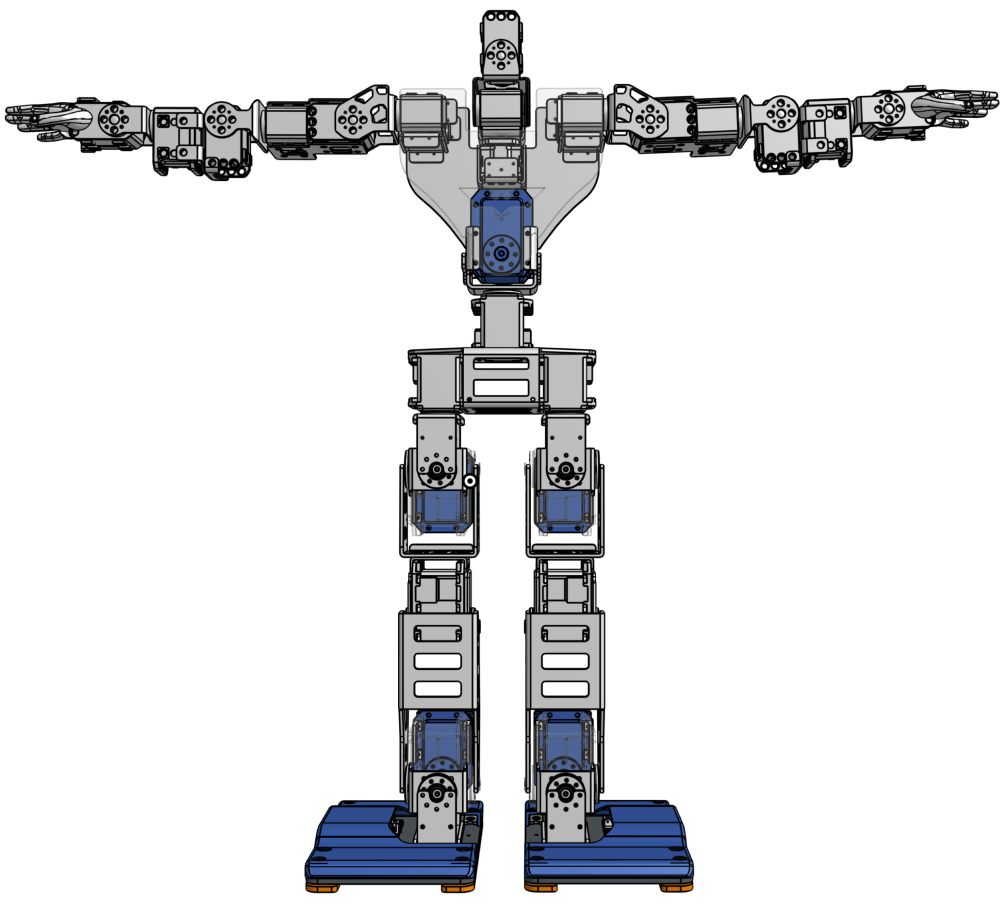
\includegraphics[width=0.4\textwidth]{gambar/controlled_servo.png}
      \caption{Servo Adjustment for Compensation Shown in Blue}
      \label{fig:Controlled_Servo}
    \end{figure}

\end{enumerate}
